\section{Thuật toán Turbo Boyer-Moore (Turbo-BM)}

\subsection{Đặc điểm chính}

Turbo-Boyer-Moore (Turbo-BM) là một biến thể cải tiến của thuật toán Boyer-Moore, được đề xuất bởi Crochemore, Czumaj, Gasieniec, Lecroq, Plandowski và Rytter vào năm 1994. Thuật toán được thiết kế nhằm giảm số phép so sánh ký tự trong quá trình tìm kiếm chuỗi bằng cách tận dụng thông tin từ các lần so khớp trước đó để tăng khoảng dịch chuyển của mẫu.

Turbo-BM kế thừa toàn bộ các heuristics của Boyer-Moore như bad-character và good-suffix, đồng thời bổ sung cơ chế turbo-shift giúp cải thiện hiệu năng trong thực tế mà không làm tăng đáng kể chi phí bộ nhớ hay tiền xử lý.

Thuật toán có các đặc điểm sau:

\begin{itemize}
    \item là một biến thể của thuật toán Boyer-Moore;
    \item không cần thêm bước tiền xử lý nào ngoài các bước của Boyer-Moore;
    \item chỉ cần thêm một lượng bộ nhớ hằng số so với Boyer-Moore;
    \item giai đoạn tiền xử lý có độ phức tạp thời gian và không gian $O(m + \sigma)$;
    \item giai đoạn tìm kiếm có độ phức tạp thời gian $O(n)$;
    \item trong trường hợp xấu nhất thực hiện không quá $2n$ phép so sánh;
\end{itemize}

\subsection{Mô tả thuật toán}

Thuật toán Turbo-BM là một cải tiến của thuật toán Boyer-Moore. Thuật toán không cần thêm bước tiền xử lý nào và chỉ yêu cầu một lượng bộ nhớ phụ hằng số so với thuật toán Boyer-Moore gốc. Ý tưởng của thuật toán là ghi nhớ đoạn của văn bản đã khớp với một hậu tố của mẫu trong lần thử trước đó (và chỉ khi thực hiện phép dịch chuyển good-suffix).

Kỹ thuật này mang lại hai lợi ích:

\begin{itemize}
    \item có thể bỏ qua đoạn đã được ghi nhớ;
    \item có thể thực hiện phép dịch chuyển turbo-shift.
\end{itemize}

Turbo-shift có thể xảy ra khi trong lần thử hiện tại, hậu tố của mẫu khớp với văn bản
ngắn hơn hậu tố đã được ghi nhớ từ lần thử trước đó. Trong trường hợp này, gọi
$u$ là đoạn đã được ghi nhớ và $v$ là hậu tố khớp trong lần thử hiện tại sao cho
$uzv$ là một hậu tố của $x$. Gọi $a$ và $b$ lần lượt là các ký tự gây ra sự không
khớp trong mẫu và văn bản ở lần thử hiện tại. Khi đó, $av$ là một hậu tố của $x$,
và do $|v| < |u|$, nên $av$ cũng là hậu tố của $u$.

Hai ký tự $a$ và $b$ xuất hiện trong văn bản với khoảng cách $p$, và hậu tố của 
$x$ có độ dài $|uzv|$ có chu kỳ độ dài $p=|zu|$ do $u$ là biên của $uzv$. Vì vậy, 
hậu tố này không thể chồng lấp lên hai lần xuất hiện của hai ký tự khác nhau $a$ 
và $b$ ở khoảng cách $p$ trong văn bản. Độ dịch chuyển nhỏ nhất có thể là
$|u| - |v|$, và độ dịch chuyển này được gọi là turbo-shift.

\begin{center}
    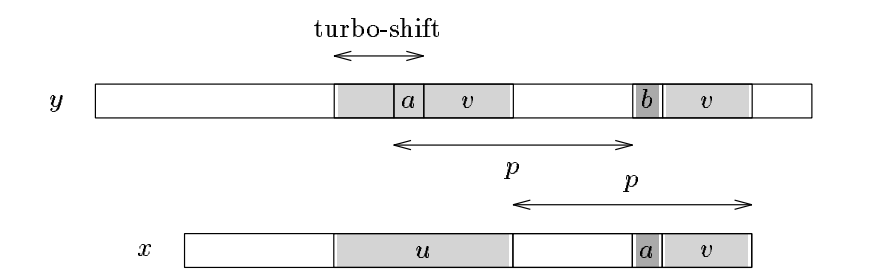
\includegraphics[width=10cm]{Images/2026-05-18-09-24-24.png}
\end{center}

Vẫn trong trường hợp $|v| - |u|$, nếu độ dài của phép dịch chuyển bad-character 
lớn hơn độ dài của phép dịch chuyển good-suffix và cả độ dài của turbo-shift, thì 
độ dài của phép dịch chuyển thực tế phải lớn hơn hoặc bằng $|u| + 1$. Thật vậy, 
trong trường hợp hai ký tự $c$ và $d$ là khác nhau, do ta giả sử rằng phép dịch chuyển 
trước đó là một phép dịch chuyển good-suffix.

\begin{center}
    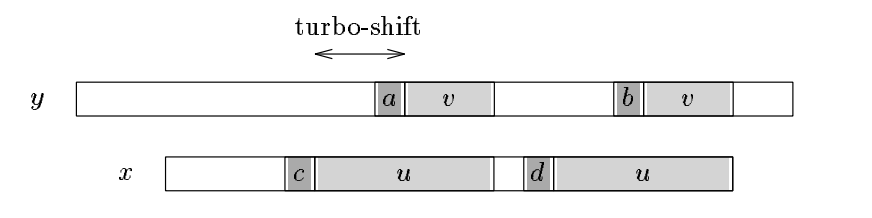
\includegraphics[width=10cm]{Images/2026-05-18-09-27-15.png}
\end{center}

Khi đó, một phép dịch chuyển lớn hơn turbo-shift nhưng nhỏ hơn $|u| + 1$ sẽ 
làm cho hai ký tự $c$ và $d$ được căn chỉnh với cùng một ký tự trong $v$. Do đó, 
trong trường hợp này, độ dài của phép dịch chuyển thực tế phải lớn hơn hoặc bằng $|u| + 1$.

Giai đoạn tiền xử lý của thuật toán có thể được thực hiện với độ phức tạp thời 
gian và không gian $O(m + \sigma)$. Giai đoạn tìm kiếm có độ phức tạp thời gian 
$O(n)$. Số phép so sánh ký tự trên văn bản mà thuật toán Turbo-Bm thực hiện bị 
chặn trên bởi $2n$.

\subsection{Cài đặt bằng C++}

\begin{verbatim}
#include <iostream>
#include <vector>
#include <string>
#include <algorithm>

using namespace std;

const int ASIZE = 256;

/* Bad Character Heuristic */
void preBmBc(const string &pat, vector<int> &bmBc) {
    int m = pat.length();

    bmBc.assign(ASIZE, m);

    for (int i = 0; i < m - 1; ++i) {
        bmBc[(unsigned char)pat[i]] = m - 1 - i;
    }
}

/* Suffixes */
void suffixes(const string &pat, vector<int> &suff) {
    int m = pat.length();

    suff.resize(m);
    suff[m - 1] = m;

    int g = m - 1;
    int f = 0;

    for (int i = m - 2; i >= 0; --i) {
        if (i > g && suff[i + m - 1 - f] < i - g) {
            suff[i] = suff[i + m - 1 - f];
        } else {
            if (i < g)
                g = i;

            f = i;

            while (g >= 0 && pat[g] == pat[g + m - 1 - f])
                --g;

            suff[i] = f - g;
        }
    }
}

/* Good Suffix Heuristic */
void preBmGs(const string &pat, vector<int> &bmGs) {
    int m = pat.length();

    vector<int> suff(m);

    suffixes(pat, suff);

    bmGs.assign(m, m);

    int j = 0;

    for (int i = m - 1; i >= 0; --i) {
        if (suff[i] == i + 1) {
            for (; j < m - 1 - i; ++j) {
                if (bmGs[j] == m)
                    bmGs[j] = m - 1 - i;
            }
        }
    }

    for (int i = 0; i <= m - 2; ++i) {
        bmGs[m - 1 - suff[i]] = m - 1 - i;
    }
}

/* Turbo Boyer-Moore */
void TBM(const string &pat, const string &txt) {
    int m = pat.length();
    int n = txt.length();

    vector<int> bmBc;
    vector<int> bmGs;

    /* Preprocessing */
    preBmBc(pat, bmBc);
    preBmGs(pat, bmGs);

    /* Searching */
    int j = 0;
    int u = 0;
    int shift = m;

    while (j <= n - m) {
        int i = m - 1;

        while (i >= 0 && pat[i] == txt[i + j]) {
            --i;

            if (u != 0 && i == m - 1 - shift)
                i -= u;
        }

        if (i < 0) {
            cout << "Pattern found at index: " << j << endl;

            shift = bmGs[0];
            u = m - shift;
        } else {
            int v = m - 1 - i;
            int turboShift = u - v;

            int bcShift =
                bmBc[(unsigned char)txt[i + j]] - m + 1 + i;

            shift = max(turboShift, bcShift);
            shift = max(shift, bmGs[i]);

            if (shift == bmGs[i]) {
                u = min(m - shift, v);
            } else {
                if (turboShift < bcShift)
                    shift = max(shift, u + 1);

                u = 0;
            }
        }

        j += shift;
    }
}

int main() {
    string text = "ABAAABCDABCABC";
    string pattern = "ABC";

    TBM(pattern, text);

    return 0;
}
\end{verbatim}

\subsection{Kiểm nghiệm thuật toán}

\begin{center}
    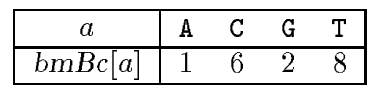
\includegraphics[width=10cm]{Images/2026-05-18-09-33-04.png}
\end{center}

\begin{center}
    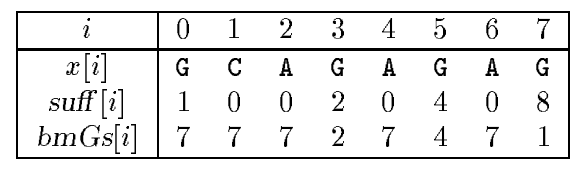
\includegraphics[width=10cm]{Images/2026-05-18-09-33-21.png}
\end{center}

\textbf{Pha tìm kiếm:}

Lần 1:

\begin{center}
    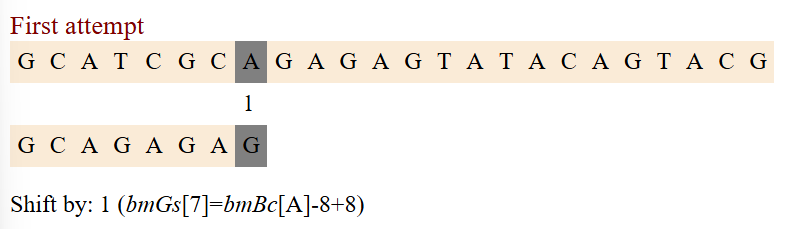
\includegraphics[width=10cm]{Images/2026-05-18-09-38-36.png}
\end{center}

Lần 2:

\begin{center}
    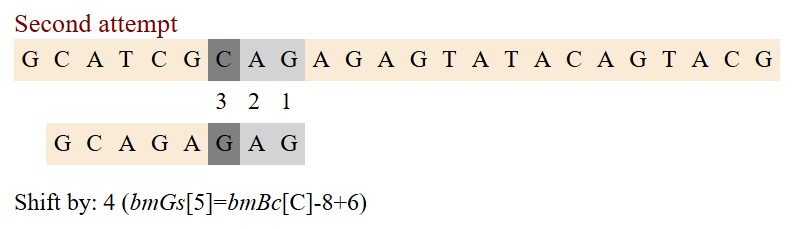
\includegraphics[width=10cm]{Images/2026-05-18-09-38-50.png}
\end{center}

Lần 3:

\begin{center}
    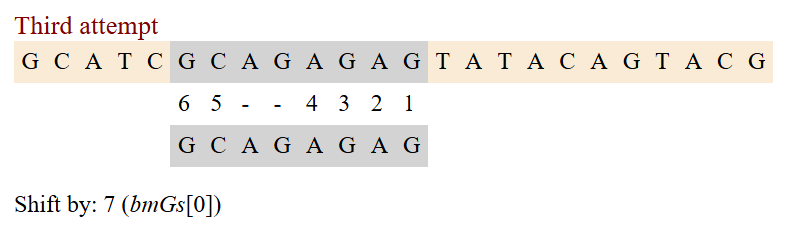
\includegraphics[width=10cm]{Images/2026-05-18-09-39-04.png}
\end{center}

Lần 4:

\begin{center}
    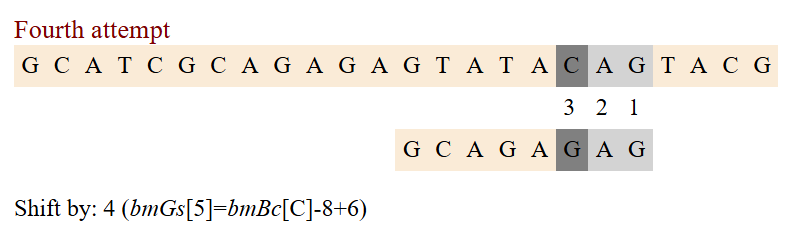
\includegraphics[width=10cm]{Images/2026-05-18-09-39-18.png}
\end{center}

Lần 5:

\begin{center}
    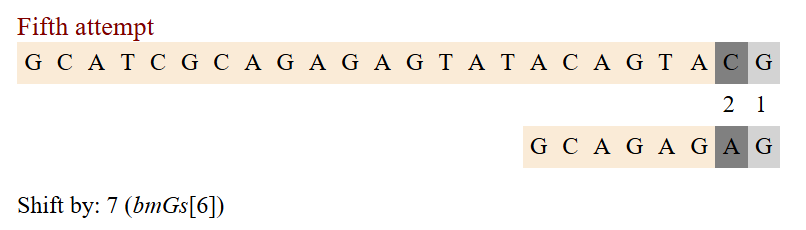
\includegraphics[width=10cm]{Images/2026-05-18-09-39-30.png}
\end{center}

Thuật toán Turbo-BM thực hiện 15 lần so sánh chuỗi trong ví dụ trên.


